\section{4D Cardiac Registration}
\label{sec:4dreg}

In order to be able to perform group analysis on a set of 4-$D$ scans of the beating heart to statistically characterize structural and functional qualities of the heart, we need to be able to perform a 4-$D$ registration between an atlas of a normal heart, the template $T$, and the subject $S$. Here 4-$D$ refers to the 4-dimensional space in which the beating heart resides, namely the regular 3-$D$ eucledean space and the 1-$D$ time space. The 4-$D$ registration will enable to to quantify the differences between a normal and an abnormal heart. Our goal is to estimate a 4-$D$ transformation that maps a given point $(\bx, t)$ in the subject to a point in the template. This transformation characterizes both the structural as well as the functional (myocardial wall motion) differences between the subject and the template. The 4-$D$ registration builds on the cardiac motion estimation algorithm described in Section \ref{sec:carMot}. The problem formulation is summarized in Figure \ref{fig:reg4d}. It is only in recent years that imaging modality acquisition technology has developed to an extent to allow us to acquire 4-$D$ datasets. These are still the early days and currently available 4-$D$ datasets are plagued by a number of problems. The three most common modalities which are used to acquire 4-$D$ datasets are MR, Ultrasound and CT. Each of these modalities have their advantages and associated problems. 
%We summarize the advantages and disadvantages of each of these in Table \ref{tab:4dmod}. These are specifically evaluated with cardiac imaging applications in mind. 
Since these modalities are so different, it is important while designing a 4-$D$ registration algorithm to keep in mind the the advantages and shortcomings of the underlying imaging modality. The features being used for correspondence detection, the energy function being minimized and the set of constraints imposed need to be carefully selected keeping the strengths of the modality in mind. Specifically, for the case of 4-$D$ image registration for cardiac applications, MR Cine sequences have been popular \cite{perperidis04}. Detecting correspondences across different patients in MR Cine sequences is not an easy task, especially for cardiac datasets, which are poor in features both because of the inherent geometry of the heart and because of shortcomings in the acquisition. 

One of the key problems when dealing with 4D MR cine sequences is that inter-slice spacing and the slice thickness are quite large. This implies that anatomical structures (features) that are imaged under one patient might not be present in the other patient's scan. This is illustrated in Figure \ref{fig:slice-thick}. This is the reason that the wavelet based attribute vectors, which evaluate the similarity in a neighborhood around the point perform much better than other local measures of similarity. 

%In the 4-$D$ case, we have additional inputs to help in correspondence detection across subject. This is the knowledge of the motion fields of the subject and the template, which have been estimated as described in Section \ref{sec:carMot}. This helps because, as the heart moves, parts of the heart that were not images earlier because of the large slice thickness, now get imaged. Therefore, by adding a constraint to keep the motion fields of the template and the subject we improve the accuracy of the correspondence detection and thereby the estimation of the 4-$D$ transform. It is also important to impose constraints that give importance to temporal consistency along with temporal smoothness. This is something that is not addressed by work already done in this field \cite{perperidis04}. We shall elaborate on these constraints later in the section.

In the 4-$D$ case, we have additional information that helps us in correspondence detection across subjects. This is the knowledge of the motion fields of the subject and the template, which can be estimated {\em a priori} as described in Section \ref{sec:carMot}. It is important to realize that if better estimates of myocardial motion are available by other means, such as tagged images or MR phase contrast imaging, they can be used directly instead of estimating the motion from the MR Cine sequences. We use the motion field to ensure that the correspondence detected between the template and the subject is consistent during the entire cardiac cycle. Apart from ensuring a temporally smooth and consistent transformation, this also helps in better correspondence detection. As the heart moves, parts of the heart that were not imaged earlier because of the large slice thickness, now get imaged. Therefore, by adding a constraint to keep the motion fields of the template and the subject consistent, we improve the accuracy of the correspondence detection and thereby the estimation of the 4-$D$ transform. It is also important to impose constraints that give importance to temporal consistency along with temporal smoothness. This is something that is not addressed by work already done in this field \cite{perperidis04}. We shall elaborate on these constraints later in the section.

\begin{figure}
\centering
     \subfigure[Points {\bf b} and {\bf d} get imaged, whereas points {\bf a} and {\bf c} do not get imaged.]{
          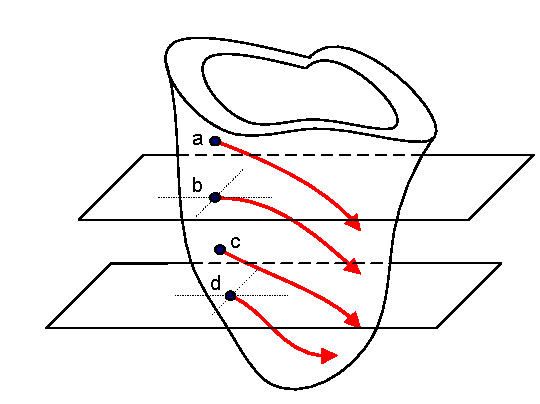
\includegraphics[width=.4\textwidth]{images/slice-thick-a}
          \label{fig:thick-a}
          }
          \hspace{.15in}
     %%\hspace{.05in}
     \subfigure[Because of cardiac motion, at a different part of the cardiac cycle, points {\bf a} and {\bf c} get imaged. However, at this time {\bf b} and {\bf d} are no longer imaged.]{
          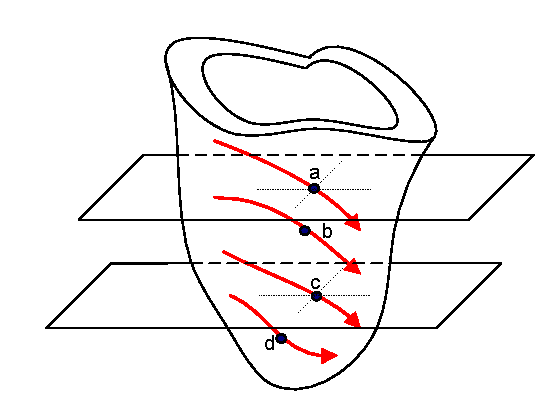
\includegraphics[width=.4\textwidth]{images/slice-thick-b}
          \label{fig:thick-b}
          }
     \caption{Imaging problems due to large inter-slice spacing}     
     \label{fig:slice-thick}
\end{figure} 

We first perform an affine registration to normalize the subject. This is essential to make the 4-$D$ transformation and consequently the classification independent of variations in sex, age, weight and height of the patient. Also the datasets might vary because of differences in the image acquisition procedure. Therefore it is extremely important to perform spatio-temporal normalization of the datasets before performing the 4-$D$ registration.

\subsection{Spatio-Temporal Affine Registration}

When registering two 4-$D$ image sequences, spatial alignment of the corresponding frames in not sufficient as the frames could correspond to different phases in the cardiac cycle of the heart. This difference arises due to,
\begin{itemize}
	\item Difference in acquisition parameters like initial offset in the acquisition of the first frame and different frequency in the acquisition of subsequent frames. 
	\item Difference in the length of the cardiac cycle, which arise due to different patients having different heart rates.
	\item Difference in the dynamic properties of the heart, i.e., differences in lengths of systole and diastole.
\end{itemize}

The spatial component of the affine transform comes due to the following differences,
\begin{itemize}
	\item Different heart sizes and orientation because of variations in sex, age, height and weight of the patient.
%	\item Difference in acquisition parameters like pixel spacing and slice thickness.
	\item Variations in the way the patient is placed inside the scanner.
\end{itemize}

Spatio-temporal alignment will enable comparison between corresponding anatomical positions and corresponding phases in the cardiac cycle of the hearts. Perperidis et al suggest a possible normalization method \cite{perperidis04} by extending their B-Spline based registration algorithm as a combination of a 3-$D$ spatial registration and a 1-$D$ temporal registration. They decouple the 4-$D$ mapping into independent spatial and temporal components. 

%\begin{table}
%	\begin{center}
%		\begin{tabular}{|c|c|c|}
%		\hline
%			Modality & Advantages & Disadvantages \\
%			\hline
%			MR & High Temporal Resolution & Low inter-slice spacing \\
%			US & Easy to acquire & Poor image information \\
%			CT & High spatial resolution (sub mm) & Poor temporal resolution \\
%			\hline
%		\end{tabular}
%	\end{center}
%
%	\caption{Comparison of current 4-$D$ modalities}
%	\label{tab:4dmod}
%\end{table}

We use a similar framework during the initial affine registration part of our 4-$D$ registration. However although it is reasonable to assume that the temporal and spatial transformations are independent, they do affect each other while estimating one with an approximate solution of the other. We do not assume that the two are independent and solve iteratively to get the optimal affine transformation. Since we are performing affine registration, it is better to use a metric that is evaluated over the entire image space. Normalized mutual information \cite{stud99} has been shown to perform well in similar registration problems. We use NMI as the similarity measure, which is given by:
\begin{equation}
NMI(A, B) = \frac{H(A) + H(B)}{H(A,B)}
\end{equation}
here $H(A)$ and $H(B)$ denote the separate entropy values of images $A$ and $B$, respectively. $H(A,B)$ is the joint entropy, i.e., the entropy of the joint probability distribution of the image intensities. We use the Shannon measure of entropy, $-\sum_{p\in P}p\log p$ for a probability distribution $P$.

First we estimate the 3D affine transformation $\mathcal{A}(\bx)$ by performing a 3D affine registration between the two end-diastole images. This is done by maximizing the normalized mutual information metric described above. We can present this as an energy minimization problem by minimizing the negative of the normalized mutual information. That is the energy that is minimized is defined as
\begin{equation}
E = -NMI(T_0(\bx), S_0(\mathcal{A}(\bx)) = -\frac{H(T_0(\bx)) + H(S_0(\mathcal{A}(\bx)))}{H(T_0(\bx),S_0(\mathcal{A}(\bx)))}
\end{equation}
where $T_0$ and $S_0$ are the end-diastole frames of the template and the subject sequences respectively.

Once this is estimated we then estimate the temporal shift and scale of the subject with respect to the template, using the estimated spatial transformation. The temporal normalization aligns the two sequences and makes the subject $S$ have the same number of frames $N$ as the template $T$. We follow this with a second set of spatial registration. The difference in this case is that the similarity is evaluated over all image pairs in the sequence. The energy function that is minimized during this step is,
\begin{equation}
E = -\sum_{i=0}^{N-1}NMI(T_i(\bx), S_i(\mathcal{A}(\bx)))=-\sum_{i=0}^{N-1}\frac{H(T_i(\bx)) + H(S_i(\mathcal{A}(\bx)))}{H(T_i(\bx),S_i(\mathcal{A}(\bx)))}
\end{equation}

Since the temporal normalization has been performed, the image pairs correspond to each other. We iterate over the last two steps till they converge and we have the final 4D affine transformation.

The results of the affine registration are shown in Figure \ref{fig:affine4d}.

\begin{figure}
     \centering
     \subfigure[The Template Image]{
          \label{fig:t1}
          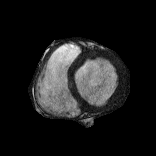
\includegraphics[width=.4\textwidth]{images/t1}}
     %%\hspace{.05in}
     \subfigure[The Subject Image]{
          \label{fig:p1}
          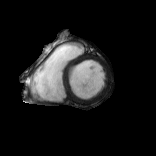
\includegraphics[width=.4\textwidth]{images/p1}} \\
     %%\hspace{.05in}
     \subfigure[The Subject warped to the template space]{
           \label{fig:affine}
           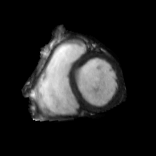
\includegraphics[width=.4\textwidth]{images/affine}}
     \caption{The result of applying the 4-D affine transform to the subject image}
     \label{fig:affine4d}
\end{figure}

%% Results of the affine registration.

In the following steps it is assumed that the subject $S$ has been warped to the template space using the results of the affine registration. Both the sequences have $N$ frames each at the end of the affine registration.

\subsection{Attribute Vector}

We use the same wavelet-attribute vector as described in Section \ref{sec:wav}. As was shown in Section \ref{sec:wav}, the wavelet attribute vectors robustly and effectively detect correspondence across patients even with deformations present. The wavelet attribute at location $( \bx, t )$ is represented as  $\bW( \bx, t )$. 

\begin{figure}
\begin{center}
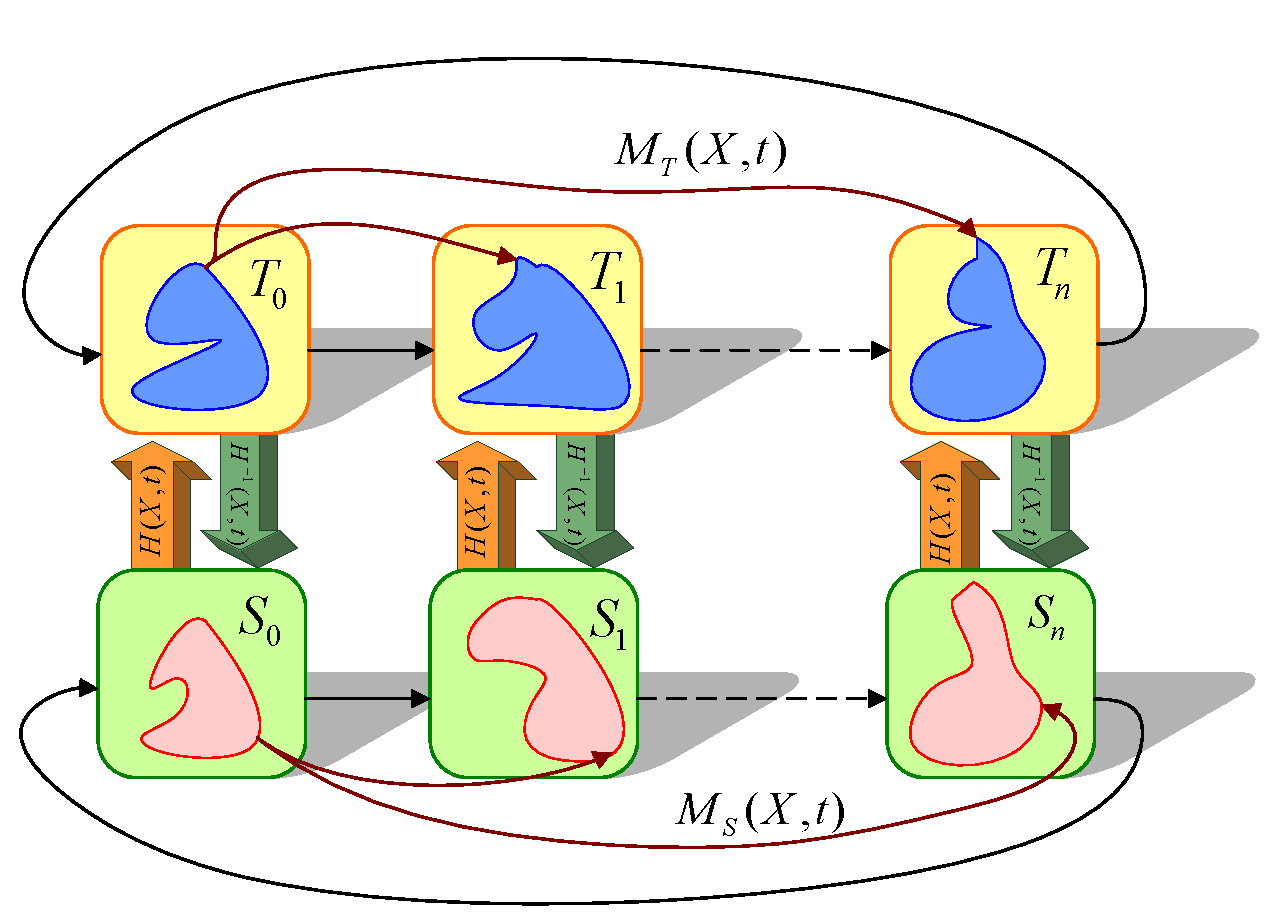
\includegraphics[width=.9\textwidth]{images/4dreg} 
\caption{Formulation of the 4D registration problem}
\label{fig:reg4d}
\end{center}
\end{figure} 

\subsection{Combined motion field extraction and 4D registration}

We now describe the algorithm for 4D registration. Since we are trying to quantify the difference between the subject $S(\bx, t)$ and the template $T(\bx, t)$, we need to compute the 4-$D$ transformation that transforms the subject to the template space. Both are 4D image sequences and the intensity at any location  $( \bx, t )$ can be accessed by, $T ( \bx, t)$ and $S ( \bx, t )$. The attribute vector $\bW$ at a given location $( \bx, t )$  is represented as $\bW_T(\bx, t)$ for the template and $\bW_S(\bx, t)$ for the subject.

We also define the following transformations:
\begin{itemize}
  \item $\bchi_T ( \bx, t )$: The motion field defined over the template
  space. The transformation maps a point $\bx$ in the end-diastole frame
  of the template to its corresponding point in frame at time $t$.
  
  \item $\bchi_S ( \bx, t )$: The motion field defined over the subject space.
  The transformation maps a point $\bx$ in the end-diastole frame of the
  subject to its corresponding point in frame at time $t$.
  
  \item $H_{T \leftarrow S} ( \bx, t )$: The 4d transformation that maps a
  4-$D$ point $( \bx, t )$ from the subject to the template space. We shall use $H ( \bx, t )$ to imply this transformation by default. The inverse transformation, $H_{S \leftarrow T} ( \bx, t )$ will be written as $H^{-1} ( \bx, t )$.
\end{itemize}
These transformations along with the formulation of the 4-$D$ registration problem are illustrated in Figure \ref {fig:reg4d}. We first compute the template motion field and the subject motion field. We then compute the 4-$D$ transformation using the two motion fields as additional constraints that help us better estimate the 4-$D$ transformation.

\subsection{Estimating the Template and Subject Motion Field}

We compute the template motion using the algorithm described in the previous section \ref{sec:CarMot}. If better estimates for the motion fields of either the subject or the template are available, say from tagged MR images or other methods, these can be used directly rather than estimating it using the method described. Depending on how much time is available for the the 4D registration, we have two strategies. The faster method is to compute the robust focus points based purely on the template image. This is done offline and needs to be done once and is therefore faster. The better albeit slower method is to compute the focus points by computing the focus points using the template and the subject, as described in Section \ref{sec:wav-distinctive}. This will need to be computed for each subject individually. A qualitative assessment will have to be done in the performance improvement in the registration as a result of using subject specific distinctiveness calculation.

\subsection{Estimation of 4D deformation field }

The problem is again posed as one of minimizing an energy function. We estimate the 4D deformation field that best maps the subject to the template and is also consistent with the template motion field $\bchi_T ( \bx, t )$ and the subject motion field $\bchi_S ( \bx, t )$. These three transformations are not independent and the two motion fields impose a strong constraint on the 4-$D$ deformation field. This relation can be expressed as:

\begin{equation}
\label{eq:4d-mot-rel}
\bchi_S ( \bx, t ) = H^{-1} ( \bchi_T ( H (\bx, 0 ), t ) )
\end{equation}

We define an energy function that incorporates the similarity between the template and the warped subject image. There is an additional energy term that is added to make the 4-$D$ transformation consistent with the two motion fields. The energy function also incorporates terms for smoothness of the deformation. The energy function that our 4D registration algorithm minimizes is defined as follows:
\begin{equation}
	E = E_F + E_B + E_C + E_{Smooth}
\end{equation}
We shall now define each of these terms in detail and the role they play in the proper estimation of the 4-$D$ transformation.

\subsubsection{Similarity}
In order to make the registration independent of which of the two sequences are treated as the template, the energy function should be symmetric to the two sequences being registered. Therefore we evaluate both the forward transformation $H^{-1} ( \bx, t )$ and the backward transformation $H ( \bx, t )$ and force them to be consistent with each other. These two evaluations give rise to the forward and backward energy terms, $E_F$ and $E_B$, respectively. These terms are defined as:
\begin{eqnarray}
  E_F &=& \sum_{t = 0}^{N - 1} \sum_{\bx \in \Omega_T }
  \eta_T ( \bx, t ) \left( \sum_{( \bz, \tau ) \in n ( \bx, t
  )} \varphi \left( \bW_T ( \bz, \tau ), \bW_S ( H^{-1} ( \bz, \tau
  ) ) \right) \right) \\
  E_B &=& \sum_{t = 0}^{N - 1} \sum_{\bx \in \Omega_S }
   \eta_S ( \bx, t ) \left( \sum_{( \bz, \tau ) \in n ( \bx,
   t )} \varphi \left( \bW_T ( H ( \bz, \tau ) ), \bW_S ( \bz,
   \tau ) \right) \right)  
\end{eqnarray}
   
The importance of each point $(\bx, t)$, in the forward energy term is determined by the corresponding parameter $\eta_T (\bx, t )$, which is designed to be proportional to the distinctiveness of the point's wavelet attribute vector $\bW_T ( \bx, t )$ on the template. Similarly the importance of each point $(\bx, t)$, in the backward energy term is determined by the corresponding parameter $\eta_S (\bx, t )$, which is designed to be proportional to the distinctiveness of the point's wavelet attribute vector $\bW_S ( \bx, t )$ on the subject. The match for each point $(\bx, t)$ is evaluated in it's 4-$D$ neighborhood $n ( \bx, t )$, by integrating the similarity measure between the attribute vector $\bW_T ( \bz, \tau )$  of every neighboring point $( \bz, \tau )$ and the attribute vector $\bW_S ( H^{-1} ( \bz, \tau ) )$  of the corresponding point in the subject. The same is true for the backward energy term. The size of the neighborhood is large initially and decreases gradually with the progress of the deformation, thereby increasing robustness and accuracy of the motion estimation. As the neighborhood size is decreased we also change the weights for the multi-resolution attribute vector's similarity, increasing the weights for the local features and decreasing the weights on the global features. Here, $\varphi(\cdot,\cdot)$ defines the similarity between two attribute vectors, as explained earlier, in Section \ref{sec:attribSim}.
   
\subsubsection{Consistency between the Motion Fields}
   
The next term in the energy function is added because in addition to maximizing the similarity between the subject and the template, we also need
that the correspondence that is implied on the subject as a result is also correct. In other words, the 4-$D$ transformation should map the same physical point from the subject to the template at all time frames. We can enforce this by adding an energy term, based on the relationship between the three transformations (\ref{eq:4d-mot-rel}). We want equation (\ref{eq:4d-mot-rel}) to be satisfied at all points across all time frames. We can therefore write the consistency energy term as,

\begin{equation}
E_C = \sum_{\bx \in \Omega_S} \sum_{t = 0}^{N - 1} \eta_S ( \bx, t ) \left( \bchi_S ( \bx, t ) - H^{-1} ( \bchi_T ( H (\bx, 0 ), t ) ) \right)^2
\end{equation}

Minimizing this energy term makes the 4-$D$ transformation as consistent with the two motion field estimates. We also weight the individual difference terms with the distinctiveness of the point, $\eta_S ( \bx, t )$.  

\subsubsection{Smoothness}
We need to ensure that the 4D deformation $H ( \bx, t )$ is smooth. We use a Laplacian term to smooth the 4D field. The level of smoothness is controlled by the factor $\zeta$. This can be written as
\begin{equation}
E_{SmoothH} = \zeta \cdot \sum_{t = 0}^{N - 1} \int_{\bx \in \Omega} \left\| \nabla^2 U ( \bx, t
   ) \right\|
\end{equation}

\subsection{Implementation Issues}

One of the key problems while dealing with 4-$D$ datasets is that of leading the datasets in memory. While registering two 4-$D$ datasets we need to have both the datasets and their attribute vectors loaded in memory, which can be a problem on most systems. Currently 32 bit architectures are limited to a maximum of 4GB of main memory. For both MS Windows and Linux, the address space higher than 3GB are reserved for the OS (Kernel memory). Therefore, it is not possible to allocate more than 3GB on these systems. One possible solutions to this problem is to switch to 64 bit architectures which allow a much larger address space. This seems reasonable since the size of medical images continues to grow and we will need more and more memory to process that much information.

Another solution could be to parallelize the energy minimization procedure. This will allow us to use clusters of 32-bit machines in a distributed way. We could load the $i$th frame of both the subject and template on the same machine\footnote{Equivalent to loading two 3-$D$ datasets} and communicate between the various nodes using message passing \cite{mpi}. This however requires a major re-implementation and parallelization of existing algorithms and code. Therefore, we intent to first evaluate the effectiveness of the algorithms proposed on 64 bit architectures before any attempt is made to parallelize the code.

\subsection{Preliminary Results}

Preliminary results of the 4D registration are shown in Figure \ref{fig:def4d}. More work needs to be done, especially concerning the regularization terms and the proper selection of the parameters to balance the similarity and the regularization terms. In addition, these results are obtained by solving only at the lower resolutions, and therefore do not capture the higher resolution changes. Once the memory related issues have been resolved it will be possible to produce better results by performing the registration at all resolutions. It can be observed that the residual effectively captures the differences that have not been succesfully captured by the transformation. More information on the residual and its use in classification will be described in the next section.

\begin{figure}
     \centering
     \subfigure[The Subject Image, frame 1]{
          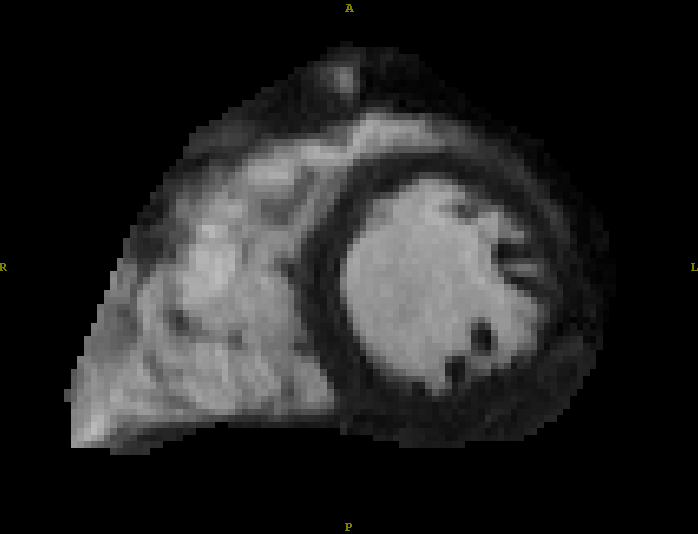
\includegraphics[width=.22\textwidth]{images/4d/p1_16}}
     \subfigure[The Subject warped to the template space]{
           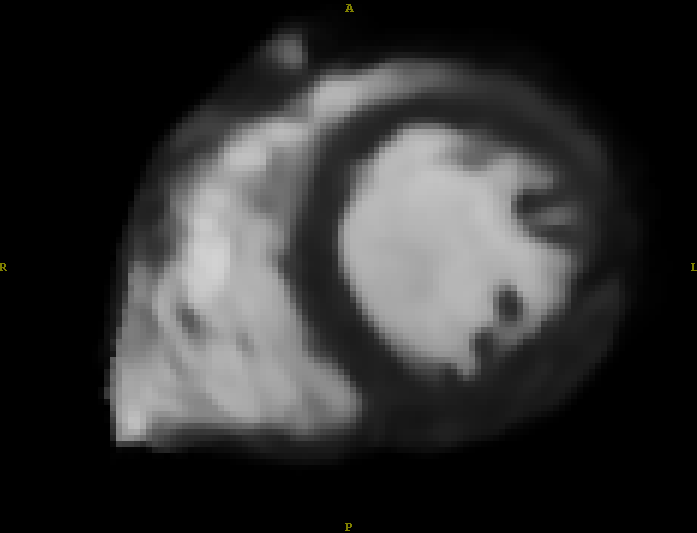
\includegraphics[width=.22\textwidth]{images/4d/warp1_16}} 
     \subfigure[The Template Image]{
          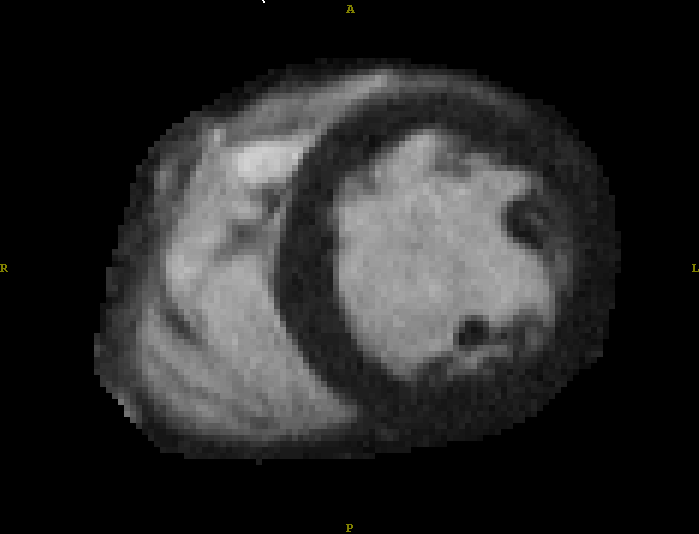
\includegraphics[width=.22\textwidth]{images/4d/t1_16}}    
     \subfigure[The Residual Image]{
          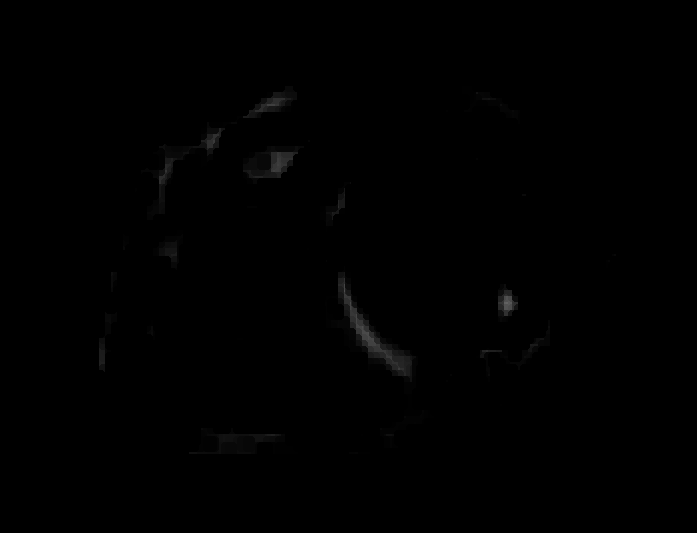
\includegraphics[width=.22\textwidth]{images/4d/r1_16}} \\
     \subfigure[The Subject Image, frame 6]{
          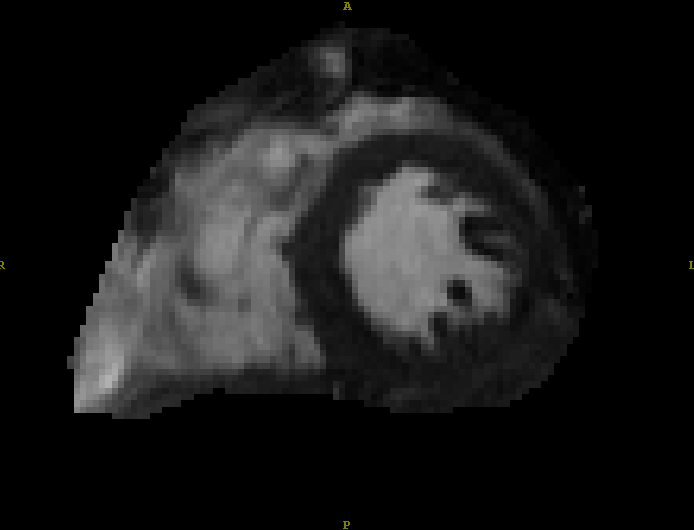
\includegraphics[width=.22\textwidth]{images/4d/p6_16}}
     \subfigure[The Subject warped to the template space]{
           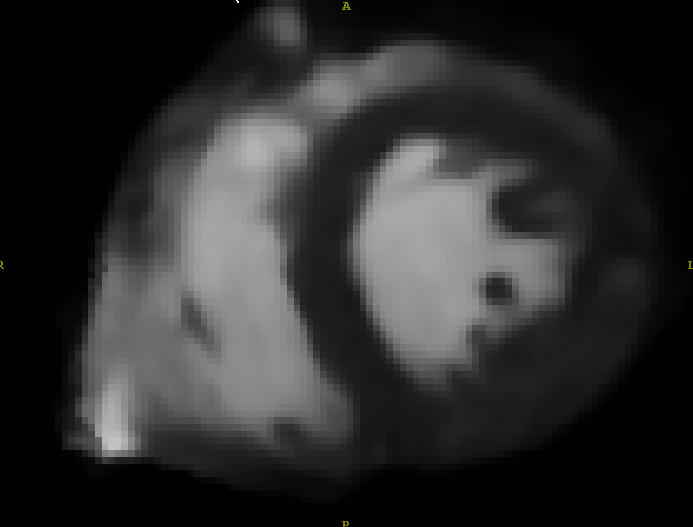
\includegraphics[width=.22\textwidth]{images/4d/warp6_16}} 
     \subfigure[The Template Image]{
          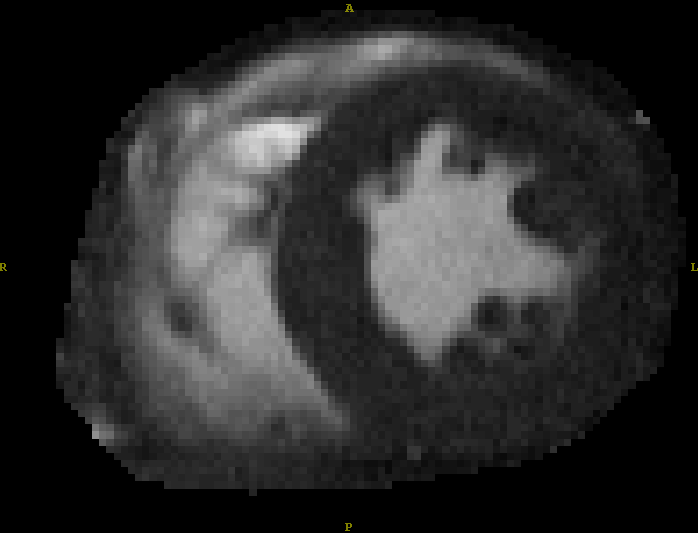
\includegraphics[width=.22\textwidth]{images/4d/t6_16}}
     \subfigure[The Residual Image]{
          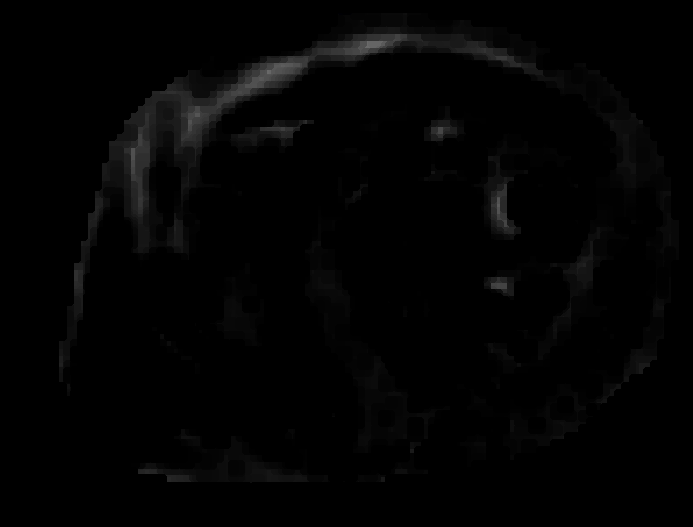
\includegraphics[width=.22\textwidth]{images/4d/r6_16}}
     \caption{Preliminary results of wavelet-attribute based deformable 4-D registration}
     \label{fig:def4d}
\end{figure}


%\subsection{Definitions}

%\begin{description}[\setlabelwidth{$\alpha\omega\pi\theta\mu$} \usemathlabelsep]
%  \item[$\gamma_T ( \vec{x}, t )$] The weights for the geometric attribute
%  vectors on the template.
  
%  \item[$\gamma_S ( \vec{x}, t )$] The weights for the geometric attribute
%  vectors on the subject.
  
%  \item[$\omega_T ( \vec{x}, t )$] The weights for the wavelet attribute
%  vectors on the template.
  
%  \item[$\omega_S ( \vec{x}, t )$] The weights for the wavelet attribute
%  vectors on the subject.
  
%  \item[$n ( \vec{x}, t )$]   The neighborhood about a point ($\vec{x}, t )$.
  
%  \item[$\varphi ( \cdot, \cdot )$]   The similarity between two attribute
%  vectors.
%\end{description}